\documentclass[english]{article}
\usepackage{graphicx}

\title{Thesis Proposal \\Textured 3D Mesh Reconstruction of Indoor Environments Using RGB-D Camera}
\author{Collin Boots}
\date{Feb 2, 2014}

\begin{document}
\maketitle
\section{Background}
As robots continue to be incorporated into human environments, the need for intelligent and high-speed reasoning about the objects around them increases dramatically. At the simplest level, mobile robots need to create a map of their environment for navigation. At a higher level, some robots need to recognize distinct objects in their environment, track object movement, and have some intuitive sense of object geometry that is easily stored and processed. Even more important is being able to efficiently generate this environment from sensor data in real time. Like the human brain, the robot should also be able to perform these low level functions with only minimal intervention from higher cognitive functions.\\
\\
RGB-D cameras provide a great low cost solution for capturing 3D environments. 3D point clouds can very quickly grow into unwieldy dense datasets filled with highly redundant data, especially in structured indoor environments with many planar surfaces. Various methods have previously been proposed to decimate point clouds using triangulation and mesh generation techniques or sparse voxel octrees (SVO). Previous work has demonstrated the diverse capabilities of depth cameras from generating highly accurate 3D surface models \cite{KinectFusion} to reliable 3D pose estimation \cite{Endres,Taguchi}. Other approaches have been able to store and merge the surface data more efficiently, but still regard the environement as a unified whole rather than discrete objects.

\section{Proposed Method}
A hybrid method is propsed that adapts existing mesh generation and triangulation techniques to online conversion of point clouds into meshes at reasonable frame rates. Each frame from the RGBD camera will be triangulated and converted to sparse meshes or incorporated into previously generated meshes. Only the decimated mesh and the current frame will need to be stored. Color data will be stored in textures allowing for very convenient processing, storage and rendering of the virtual environment. To achieve the processing speed required by the meshing pipeline, a high percentage of the processing work will be offloaded to the GPU.


By extracting meaningful geometry from the RGB-D in the form of triangle meshes, a large number of advantages can be realized.
\begin{enumerate}
\item The storage format of a trinagle mesh is very efficient, allowing for large and detailed maps to be stored in memory constrained systems like small mobile robots. 
\item Mesh models provide a natural way of isolating distinct objects in the environment in a way that point clouds and surface maps cannot. 
\item Meshes are easy to manipulate, modify, and maintain in real time using well established computer graphics technology and open the problem to the wealth of domain knowledge from the gaming graphics industry. By representing the robot's environment in a similar manner to a game world, future robots may be able to more easily leverage the gaming industry's experience in intelligent actor design. 
\item By manipulating and moving meshes instead of erasing and redrawing portions of a discrete map or point cloud, map artifacts from more dynamic environements could be handled more gracefully and naturally.
\item Storing objects as distinct, flexible models provides a natural means of handling moving objects in lower level software, freeing higher level processes for reasonsing about object movement more abstractly.
\item Meshes provide an efficient and easy to process intuition of geometry to higher cognitive functions that may simply object recognition and manipulation tasks.
\item Meshes are very flexible in their ability to record complex geometries. By using a single storage format for all object types, many implementation efficiencies may be realized. Also, meshes provide a very straightforward tradeoff between simplicity and accuracy that can be controlled dynamically.
\end{enumerate}
Using an off the shelf RGB-D depth camera like the Kinect to accomplish all of these goals also brings with it all the benefits explored in previous work: hardware simplicity, minimal integration complexity, and low cost. This work will focus primarily on generation of high-accuracy triangle meshes for a variety of scene complexities and difficult edge cases such as touching objects. Time and technology permitting, some of the potential advantages of the approach listed above will be explored and demonstrated.

\section{System Design Overview}
\begin{figure}[systemdiagram]
    \centering
    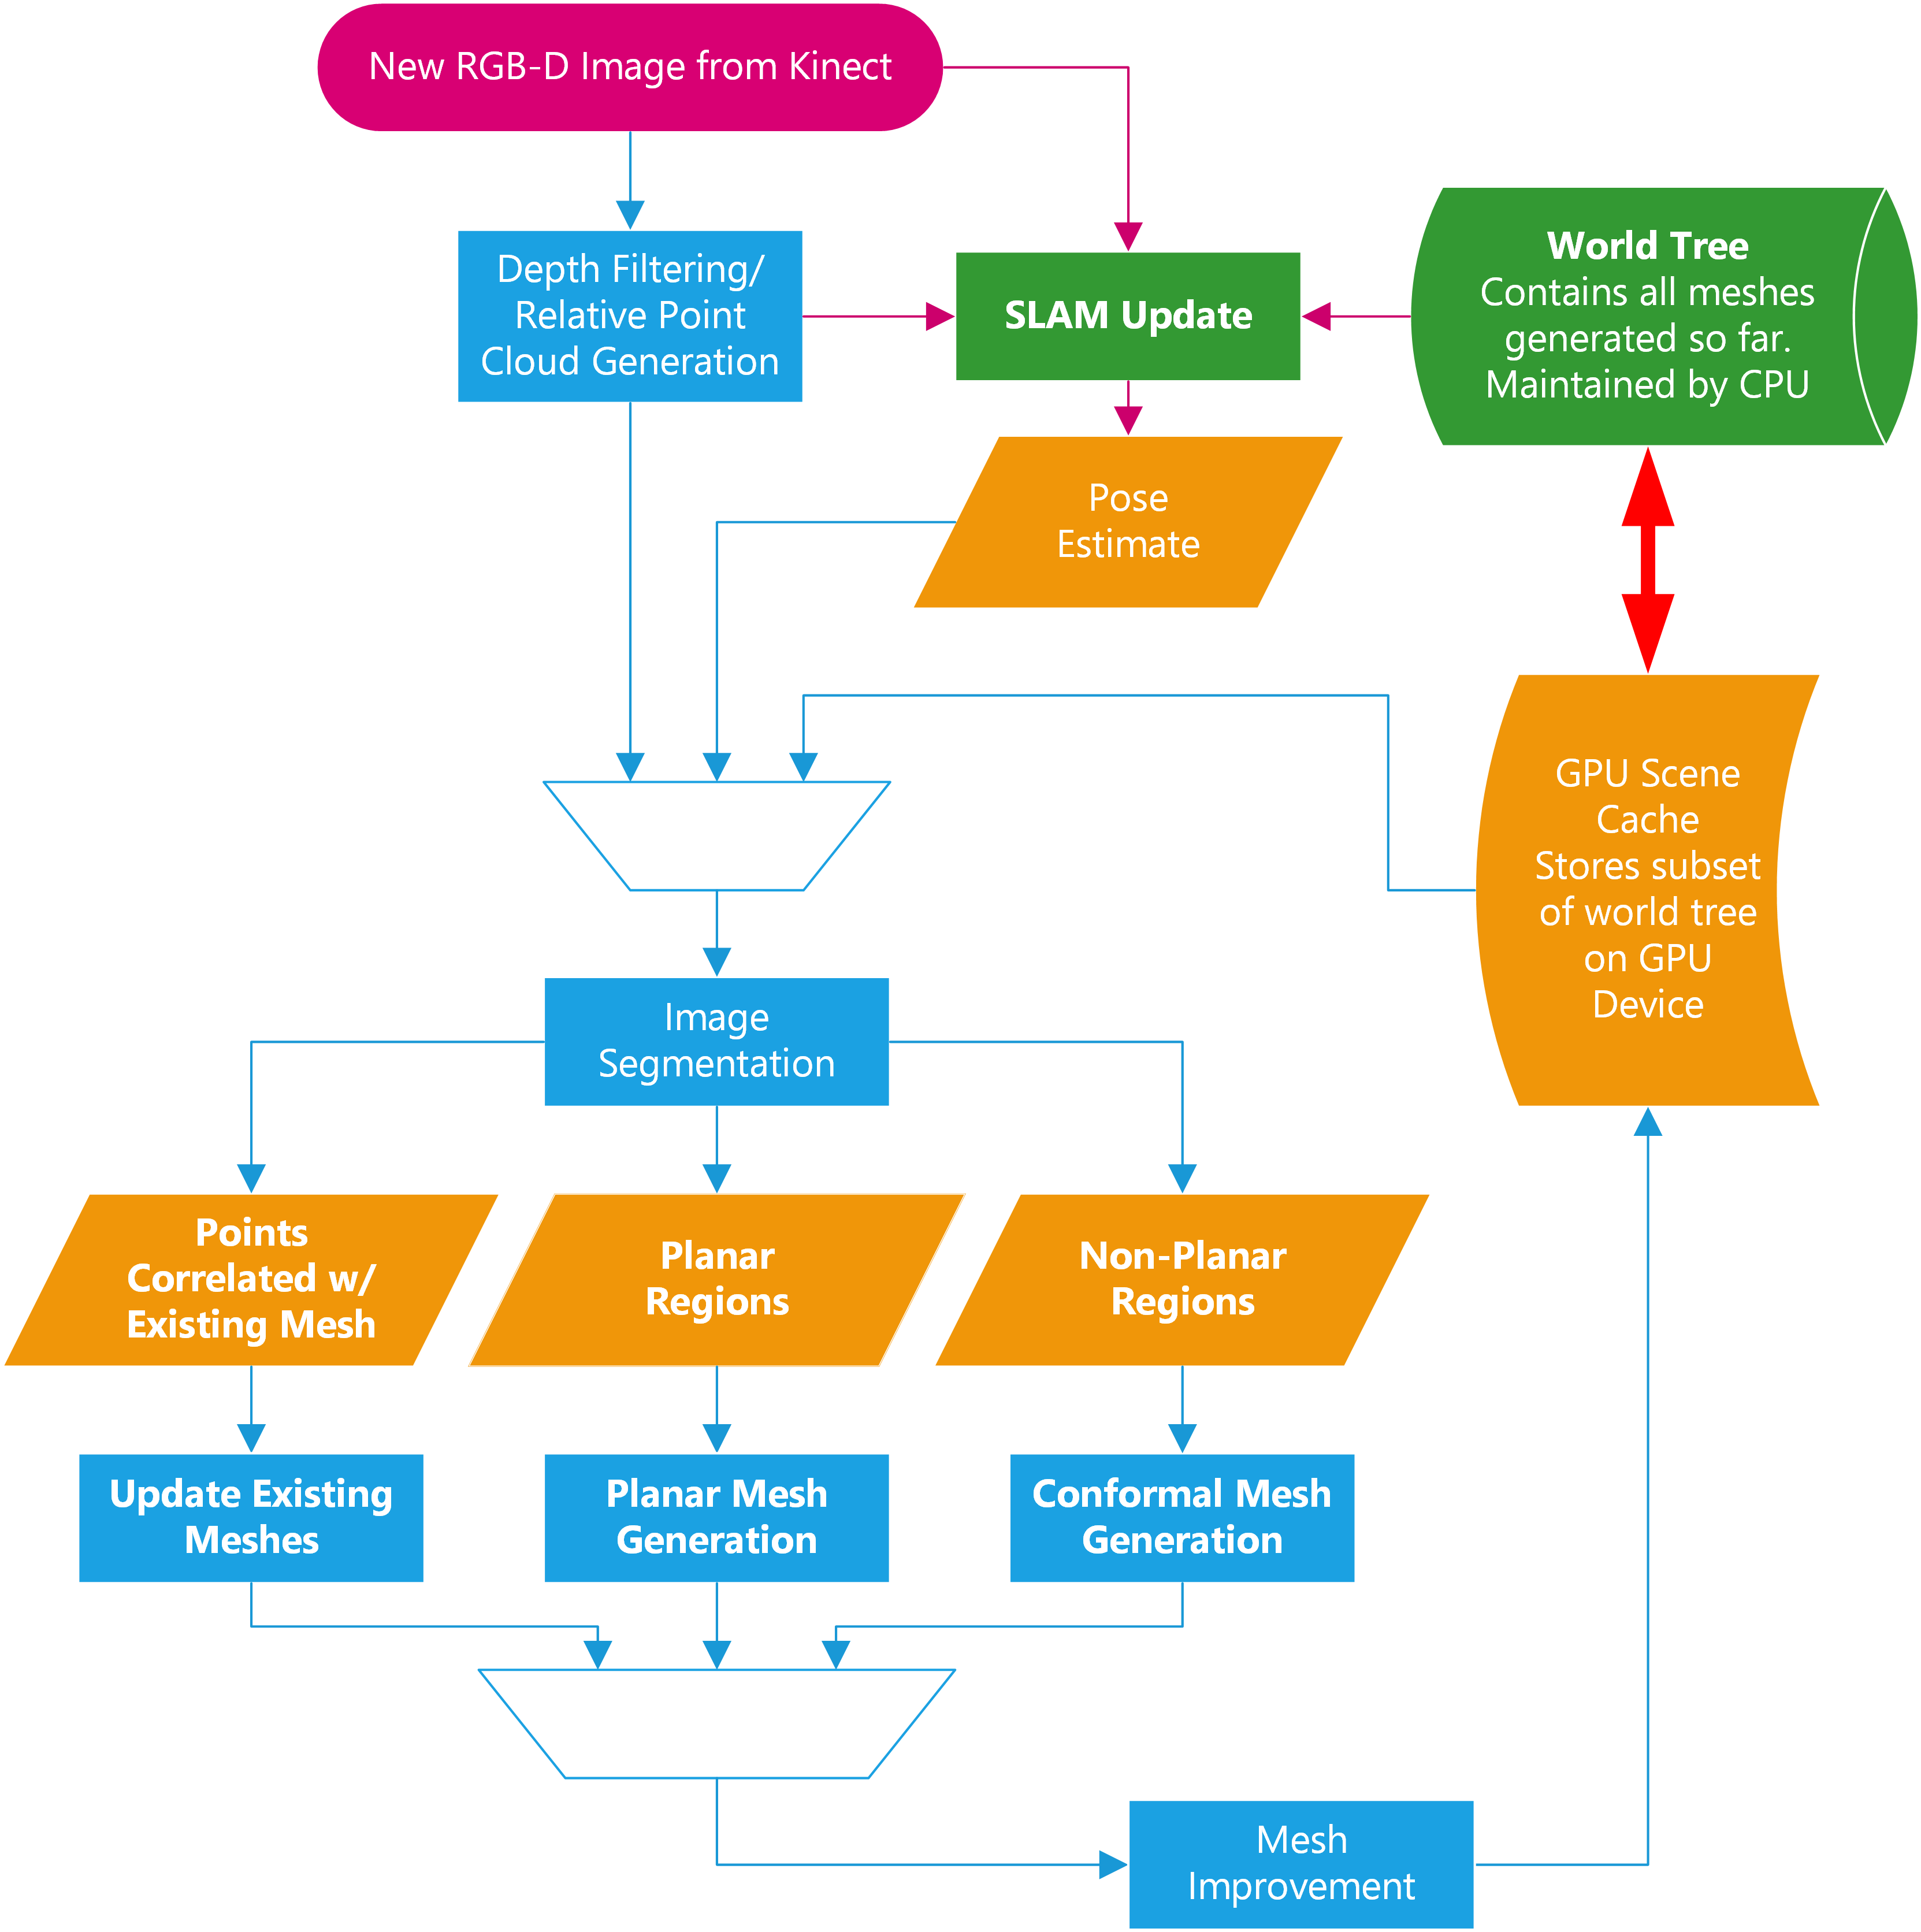
\includegraphics[width=0.8\textwidth]{Diagrams/TopLevelPipeline.png}
    \caption{System Level Data Flow Pipeline}
    \label{fig:systemdiagram}
\end{figure}

Figure~\ref{fig:systemdiagram} outlines the processing pipeline from raw RGB-D image inputs to the finished world tree representation at a very high level. 

\subsection{World Tree}
The world tree will be maintained in main computer memory by the CPU. It will store the complete mesh representation of the world in a hierarchical tree data structure similar to a scene graph. Unlike a generic scene graph, this structure will be maintained as a strict tree. Each leaf node will contain a single mesh object. Each mesh's component verticies will be stored in an object local reference frame. Objects will be transfromed into world space through a series of transformations stored in each node of the tree. This system allows objects to be easily grouped for efficient rendering and simple manipulation.

\subsection{GPU World Cache}
To reduce data redundancy and GPU memory usage, the GPU will only have direct access to a device cached subset of the world tree. The optimal heuristics for maintaining the integrety and efficiency have not been developed yet, but the goal is to maintain a GPU copy of all known meshes in the Kinect's current field of view and those likely to come into view in the next few frames. The cache synchronization with the world tree and subset selection will be handled by the CPU.

\subsection{Input Processing and SLAM}
The raw RGB-D image from the kinect sensor is first passed to the GPU so the data can be filtered and processed in parallel. Simultaneously, the CPU processes the 2D features required for the SLAM pose update step. Once the data is processed, the SLAM algrotihm will complete its pose estimation processing, combining the current world model as stored in the world tree, the 2D features computed previously, and the 3D features from the newly generated point cloud.

\subsection{Image Segmentation}

This will be one of the most challenging aspects of the pipeline to implement. Using a combination of information from the processed RGB-D frame, the current camera pose estimate, and the GPU cached world model, each point in the frame's point cloud will be segmented into three categories: points that correspond to parts of the existing mesh world, uncorrelated planar regions, and uncorrelated non-planar regions. Each category will be processed very differently at the next stage, so generating a robust segmentation will be crucial. Within each category, individual regions will be indexed so they can be easily processed in a region parallel manner for the meshing stage.

\subsection{Meshing}
Each region generated by the segmentation stage will be processed in parallel and in a very different way.
\subsubsection{Correlated Points}
Points that were determined to correspond to existing meshes will be used to update the existing meshes. Points will be used to add new verticies to a mesh as needed for added detail or to increase confidence in existing vertex estimates. This process allows the pipeline to take full advantage of higher resolution/closer capture frames of previously seen meshes. RGB data will also be used to update model texturing, allowing for texture quality improvement.

\subsubsection{Planar Regions}
Planar regions will be projected to a best-fit true plane and triangulated using a QuadTree-Based (QTB) triangulation algorithm developed in \cite{planesegmentationQTB}. The method has been demonstrated to efficiently decimate points clouds and dramatically simplifies triangulation and texture generations. If a planar region is determined to overlap with an existing plane, the existing quad-tree will be expanded to encorporate the new information.

\subsubsection{Non-planar Regions}
The remaining regions will be triangulated and converted into a new non-planar mesh object using simple polygon based triangulation method. Since conforming texture generation with arbitrary surfaces is a difficult problem to solve in real time with minimal distortion, non-planar meshes will be vertex colored. With a detailed enough triangulation, the visual quality of the of vertex shading is comparable to a textured mesh. The framework would allow for simple addition of textures later if a texture would be a more efficient representation.

\subsection{Mesh Improvement}
Once individual mesh regions have been generated, meshes are checked for easy optimizations and the potential for mesh merging. The goal of this stage is to reduce the number of verticies and distinct objects. This step is optional and not required for the pipeline to function, but it can help to simplify the representation.


\bibliographystyle{plain}
\bibliography{Sources}
\end{document}
